\documentclass{article}

\usepackage{amsmath}
\usepackage{array}
\usepackage{bm}
\usepackage[shortlabels]{enumitem}
\usepackage{graphicx}
\usepackage{hyperref}
\usepackage{interval}
\usepackage{listings}
\usepackage{pdflscape}
\usepackage{physics}
\usepackage{rotating}
\usepackage{struktex}
\usepackage{tabularx}
\usepackage{tikz}
\usetikzlibrary{positioning}
\usepackage{xcolor}
\definecolor{light-gray}{gray}{.9}
\usepackage{xfrac}

\newcolumntype{M}{>{\centering\arraybackslash}m{.3cm}}

\newcommand{\rot}[1]{\rotatebox{90}{#1}}

\author{
  Albina Oscherowa \\
  Karsten Lehmann
}
\date{WiSe 2020}
\title{Hausaufgaben Programmieren - Grundlegende Konzepte (PR10)}

\begin{document}
\maketitle

\newpage
\begin{landscape}    
  \section*{Aufgabe 6}
  
  \begin{enumerate}[a)]
  \item
    \begin{tiny}
    \[
      \begin{array}{c | MMMMMMMMMMMMMMMMMMMMMMMMMMMMMMMM}
        m_x * 2^{e_x} & \rot{0.00000} & \rot{0.00001} & \rot{0.00010} & \rot{0.00011} & \rot{0.00100} & \rot{0.00101} & \rot{0.00110} & \rot{0.00111} & \rot{0.01000} & \rot{0.01001} & \rot{0.01010} & \rot{0.01011} & \rot{0.01100} & \rot{0.01101} & \rot{0.01110} & \rot{0.01111} & \rot{0.10000} & \rot{0.10001} & \rot{0.10010} & \rot{0.10011} & \rot{0.10100} & \rot{0.10101} & \rot{0.10110} & \rot{0.10111} & \rot{0.11000} & \rot{0.11001} & \rot{0.11010} & \rot{0.11011} & \rot{0.11100} & \rot{0.11101} & \rot{0.11110} & \rot{0.11111} \\
        \hline
        e_x = -1 & 0 & \sfrac{1}{64} & \sfrac{1}{32} & \sfrac{3}{64} & \sfrac{1}{16} & \sfrac{5}{64} & \sfrac{3}{32} & \sfrac{7}{64} & \sfrac{1}{8} & \sfrac{9}{64} & \sfrac{5}{32} & \sfrac{11}{64} & \sfrac{3}{16} & \sfrac{13}{64} & \sfrac{7}{32} & \sfrac{15}{64} & \sfrac{1}{4} & \sfrac{17}{64} & \sfrac{9}{32} & \sfrac{19}{64} & \sfrac{5}{16} & \sfrac{21}{64} & \sfrac{11}{32} & \sfrac{23}{64} & \sfrac{3}{8} & \sfrac{25}{64} & \sfrac{13}{32} & \sfrac{27}{64} & \sfrac{7}{16} & \sfrac{29}{64} & \sfrac{15}{32} & \sfrac{31}{64} \\
        e_x = 0 & 0 & \sfrac{1}{32} & \sfrac{1}{16} & \sfrac{3}{32} & \sfrac{1}{8} & \sfrac{5}{32} & \sfrac{3}{16} & \sfrac{7}{32} & \sfrac{1}{4} & \sfrac{9}{32} & \sfrac{5}{16} & \sfrac{11}{32} & \sfrac{3}{8} & \sfrac{13}{32} & \sfrac{7}{16} & \sfrac{15}{32} & \sfrac{1}{2} & \sfrac{17}{32} & \sfrac{9}{16} & \sfrac{19}{32} & \sfrac{5}{8} & \sfrac{21}{32} & \sfrac{11}{16} & \sfrac{23}{32} & \sfrac{3}{4} & \sfrac{25}{32} & \sfrac{13}{16} & \sfrac{27}{32} & \sfrac{7}{8} & \sfrac{29}{32} & \sfrac{15}{16} & \sfrac{31}{32} \\
        e_x = 1 & 0 & \sfrac{1}{16} & \sfrac{1}{8} & \sfrac{3}{16} & \sfrac{1}{4} & \sfrac{5}{16} & \sfrac{3}{8} & \sfrac{7}{16} & \sfrac{1}{2} & \sfrac{9}{16} & \sfrac{5}{8} & \sfrac{11}{16} & \sfrac{3}{4} & \sfrac{13}{16} & \sfrac{7}{8} & \sfrac{15}{16} & 1 & \sfrac{17}{16} & \sfrac{9}{8} & \sfrac{19}{16} & \sfrac{5}{4} & \sfrac{21}{16} & \sfrac{11}{8} & \sfrac{23}{16} & \sfrac{3}{2} & \sfrac{25}{16} & \sfrac{13}{8} & \sfrac{27}{16} & \sfrac{7}{4} & \sfrac{29}{16} & \sfrac{15}{8} & \sfrac{31}{16} \\
        e_x = 2 & 0 & \sfrac{1}{8} & \sfrac{1}{4} & \sfrac{3}{8} & \sfrac{1}{2} & \sfrac{5}{8} & \sfrac{3}{4} & \sfrac{7}{8} & 1 & \sfrac{9}{8} & \sfrac{5}{4} & \sfrac{11}{8} & \sfrac{3}{2} & \sfrac{13}{8} & \sfrac{7}{4} & \sfrac{15}{8} & 2 & \sfrac{17}{8} & \sfrac{9}{4} & \sfrac{19}{8} & \sfrac{5}{2} & \sfrac{21}{8} & \sfrac{11}{4} & \sfrac{23}{8} & 3 & \sfrac{25}{8} & \sfrac{13}{4} & \sfrac{27}{8} & \sfrac{7}{2} & \sfrac{29}{8} & \sfrac{15}{4} & \sfrac{31}{8} \\
      \end{array}
    \]
    \end{tiny}
  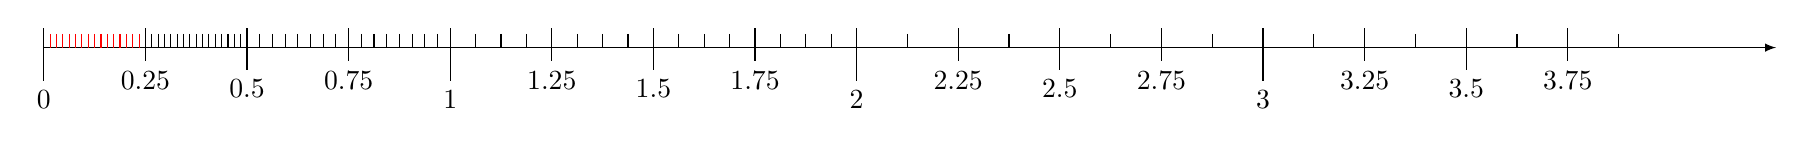
\begin{tikzpicture}
    \coordinate (c0) at (0,0);
    \coordinate (c1) at (22,0);
    \draw[-latex] (c0) -> (c1);
    \draw[red,shift={(0.0,0)}] (0pt,5pt) -- (0pt,0pt);
    \draw[shift={(0.0,0)}] (0pt,7pt) -- (0pt,-12pt) node[below] {0};
    \draw[red,shift={(0.08064516129032258,0)}] (0pt,5pt) -- (0pt,0pt);
    \draw[red,shift={(0.16129032258064516,0)}] (0pt,5pt) -- (0pt,0pt);
    \draw[red,shift={(0.24193548387096775,0)}] (0pt,5pt) -- (0pt,0pt);
    \draw[red,shift={(0.3225806451612903,0)}] (0pt,5pt) -- (0pt,0pt);
    \draw[red,shift={(0.4032258064516129,0)}] (0pt,5pt) -- (0pt,0pt);
    \draw[red,shift={(0.4838709677419355,0)}] (0pt,5pt) -- (0pt,0pt);
    \draw[red,shift={(0.564516129032258,0)}] (0pt,5pt) -- (0pt,0pt);
    \draw[red,shift={(0.6451612903225806,0)}] (0pt,5pt) -- (0pt,0pt);
    \draw[red,shift={(0.7258064516129032,0)}] (0pt,5pt) -- (0pt,0pt);
    \draw[red,shift={(0.8064516129032258,0)}] (0pt,5pt) -- (0pt,0pt);
    \draw[red,shift={(0.8870967741935484,0)}] (0pt,5pt) -- (0pt,0pt);
    \draw[red,shift={(0.967741935483871,0)}] (0pt,5pt) -- (0pt,0pt);
    \draw[red,shift={(1.0483870967741935,0)}] (0pt,5pt) -- (0pt,0pt);
    \draw[red,shift={(1.129032258064516,0)}] (0pt,5pt) -- (0pt,0pt);
    \draw[red,shift={(1.2096774193548387,0)}] (0pt,5pt) -- (0pt,0pt);
    \draw[shift={(1.2903225806451613,0)}] (0pt,5pt) -- (0pt,0pt);
    \draw[shift={(1.2903225806451613,0)}] (0pt,7pt) -- (0pt,-5pt) node[below] {0.25};
    \draw[shift={(1.3709677419354838,0)}] (0pt,5pt) -- (0pt,0pt);
    \draw[shift={(1.4516129032258065,0)}] (0pt,5pt) -- (0pt,0pt);
    \draw[shift={(1.532258064516129,0)}] (0pt,5pt) -- (0pt,0pt);
    \draw[shift={(1.6129032258064515,0)}] (0pt,5pt) -- (0pt,0pt);
    \draw[shift={(1.6935483870967742,0)}] (0pt,5pt) -- (0pt,0pt);
    \draw[shift={(1.7741935483870968,0)}] (0pt,5pt) -- (0pt,0pt);
    \draw[shift={(1.8548387096774193,0)}] (0pt,5pt) -- (0pt,0pt);
    \draw[shift={(1.935483870967742,0)}] (0pt,5pt) -- (0pt,0pt);
    \draw[shift={(2.0161290322580645,0)}] (0pt,5pt) -- (0pt,0pt);
    \draw[shift={(2.096774193548387,0)}] (0pt,5pt) -- (0pt,0pt);
    \draw[shift={(2.1774193548387095,0)}] (0pt,5pt) -- (0pt,0pt);
    \draw[shift={(2.258064516129032,0)}] (0pt,5pt) -- (0pt,0pt);
    \draw[shift={(2.338709677419355,0)}] (0pt,5pt) -- (0pt,0pt);
    \draw[shift={(2.4193548387096775,0)}] (0pt,5pt) -- (0pt,0pt);
    \draw[shift={(2.5,0)}] (0pt,5pt) -- (0pt,0pt);
    \draw[shift={(2.5806451612903225,0)}] (0pt,5pt) -- (0pt,0pt);
    \draw[shift={(2.5806451612903225,0)}] (0pt,7pt) -- (0pt,-8pt) node[below] {0.5};
    \draw[shift={(2.7419354838709675,0)}] (0pt,5pt) -- (0pt,0pt);
    \draw[shift={(2.903225806451613,0)}] (0pt,5pt) -- (0pt,0pt);
    \draw[shift={(3.064516129032258,0)}] (0pt,5pt) -- (0pt,0pt);
    \draw[shift={(3.225806451612903,0)}] (0pt,5pt) -- (0pt,0pt);
    \draw[shift={(3.3870967741935485,0)}] (0pt,5pt) -- (0pt,0pt);
    \draw[shift={(3.5483870967741935,0)}] (0pt,5pt) -- (0pt,0pt);
    \draw[shift={(3.7096774193548385,0)}] (0pt,5pt) -- (0pt,0pt);
    \draw[shift={(3.870967741935484,0)}] (0pt,5pt) -- (0pt,0pt);
    \draw[shift={(3.870967741935484,0)}] (0pt,7pt) -- (0pt,-5pt) node[below] {0.75};
    \draw[shift={(4.032258064516129,0)}] (0pt,5pt) -- (0pt,0pt);
    \draw[shift={(4.193548387096774,0)}] (0pt,5pt) -- (0pt,0pt);
    \draw[shift={(4.354838709677419,0)}] (0pt,5pt) -- (0pt,0pt);
    \draw[shift={(4.516129032258064,0)}] (0pt,5pt) -- (0pt,0pt);
    \draw[shift={(4.67741935483871,0)}] (0pt,5pt) -- (0pt,0pt);
    \draw[shift={(4.838709677419355,0)}] (0pt,5pt) -- (0pt,0pt);
    \draw[shift={(5.0,0)}] (0pt,5pt) -- (0pt,0pt);
    \draw[shift={(5.161290322580645,0)}] (0pt,5pt) -- (0pt,0pt);
    \draw[shift={(5.161290322580645,0)}] (0pt,7pt) -- (0pt,-12pt) node[below] {1};
    \draw[shift={(5.483870967741935,0)}] (0pt,5pt) -- (0pt,0pt);
    \draw[shift={(5.806451612903226,0)}] (0pt,5pt) -- (0pt,0pt);
    \draw[shift={(6.129032258064516,0)}] (0pt,5pt) -- (0pt,0pt);
    \draw[shift={(6.451612903225806,0)}] (0pt,5pt) -- (0pt,0pt);
    \draw[shift={(6.451612903225806,0)}] (0pt,7pt) -- (0pt,-5pt) node[below] {1.25};
    \draw[shift={(6.774193548387097,0)}] (0pt,5pt) -- (0pt,0pt);
    \draw[shift={(7.096774193548387,0)}] (0pt,5pt) -- (0pt,0pt);
    \draw[shift={(7.419354838709677,0)}] (0pt,5pt) -- (0pt,0pt);
    \draw[shift={(7.741935483870968,0)}] (0pt,5pt) -- (0pt,0pt);
    \draw[shift={(7.741935483870968,0)}] (0pt,7pt) -- (0pt,-8pt) node[below] {1.5};
    \draw[shift={(8.064516129032258,0)}] (0pt,5pt) -- (0pt,0pt);
    \draw[shift={(8.387096774193548,0)}] (0pt,5pt) -- (0pt,0pt);
    \draw[shift={(8.709677419354838,0)}] (0pt,5pt) -- (0pt,0pt);
    \draw[shift={(9.032258064516128,0)}] (0pt,5pt) -- (0pt,0pt);
    \draw[shift={(9.032258064516128,0)}] (0pt,7pt) -- (0pt,-5pt) node[below] {1.75};
    \draw[shift={(9.35483870967742,0)}] (0pt,5pt) -- (0pt,0pt);
    \draw[shift={(9.67741935483871,0)}] (0pt,5pt) -- (0pt,0pt);
    \draw[shift={(10.0,0)}] (0pt,5pt) -- (0pt,0pt);
    \draw[shift={(10.32258064516129,0)}] (0pt,5pt) -- (0pt,0pt);
    \draw[shift={(10.32258064516129,0)}] (0pt,7pt) -- (0pt,-12pt) node[below] {2};
    \draw[shift={(10.96774193548387,0)}] (0pt,5pt) -- (0pt,0pt);
    \draw[shift={(11.612903225806452,0)}] (0pt,5pt) -- (0pt,0pt);
    \draw[shift={(11.612903225806452,0)}] (0pt,7pt) -- (0pt,-5pt) node[below] {2.25};
    \draw[shift={(12.258064516129032,0)}] (0pt,5pt) -- (0pt,0pt);
    \draw[shift={(12.903225806451612,0)}] (0pt,5pt) -- (0pt,0pt);
    \draw[shift={(12.903225806451612,0)}] (0pt,7pt) -- (0pt,-8pt) node[below] {2.5};
    \draw[shift={(13.548387096774194,0)}] (0pt,5pt) -- (0pt,0pt);
    \draw[shift={(14.193548387096774,0)}] (0pt,5pt) -- (0pt,0pt);
    \draw[shift={(14.193548387096774,0)}] (0pt,7pt) -- (0pt,-5pt) node[below] {2.75};
    \draw[shift={(14.838709677419354,0)}] (0pt,5pt) -- (0pt,0pt);
    \draw[shift={(15.483870967741936,0)}] (0pt,5pt) -- (0pt,0pt);
    \draw[shift={(15.483870967741936,0)}] (0pt,7pt) -- (0pt,-12pt) node[below] {3};
    \draw[shift={(16.129032258064516,0)}] (0pt,5pt) -- (0pt,0pt);
    \draw[shift={(16.774193548387096,0)}] (0pt,5pt) -- (0pt,0pt);
    \draw[shift={(16.774193548387096,0)}] (0pt,7pt) -- (0pt,-5pt) node[below] {3.25};
    \draw[shift={(17.419354838709676,0)}] (0pt,5pt) -- (0pt,0pt);
    \draw[shift={(18.064516129032256,0)}] (0pt,5pt) -- (0pt,0pt);
    \draw[shift={(18.064516129032256,0)}] (0pt,7pt) -- (0pt,-8pt) node[below] {3.5};
    \draw[shift={(18.70967741935484,0)}] (0pt,5pt) -- (0pt,0pt);
    \draw[shift={(19.35483870967742,0)}] (0pt,5pt) -- (0pt,0pt);
    \draw[shift={(19.35483870967742,0)}] (0pt,7pt) -- (0pt,-5pt) node[below] {3.75};
    \draw[shift={(20.0,0)}] (0pt,5pt) -- (0pt,0pt);
  \end{tikzpicture}

  \color{red} Denormalisierte Gleitkommazahlen \color{black} Normalisierte Gleitkommazahlen
    
 \end{enumerate}
\end{landscape}
\newpage
\begin{enumerate}[a)]
\setcounter{enumi}{1}
\item
  \begin{enumerate}[1)]
  \item
    $3_{10} = 11_{2}$
    \begin{align*}
      0.875 * 2 &= \framebox{1}.75 \\
      0.75  * 2 &= \framebox{1}.5 \\
      0.5   * 2 &= \framebox{1}.0 \\
    \end{align*}
    $3.875_{10} = 11.111_{2}$
    
    \begin{minipage}[t]{.4\textwidth}
      \[
        \begin{array}{cccc cccc c}
          0.&1&1&1&*&1&0&1&0 \\
          \cline{0-8}
            & & & & & &0&0&0 \\
            & & & & &1&1&1 \\
            & & & &0&0&0 \\
            & & &1&1&1 \\
          \cline{0-8}
          \bm{8}&=&\bm{0}&\bm{1}&\bm{0}&\bm{0}.&1&1&0 \\
        \end{array}
      \]
    \end{minipage}
    \hfill
    \begin{minipage}[t]{.4\textwidth}
      \[
        \begin{array}{cccc cccc}
          0.&1&1&*&1&0&1&0 \\
          \cline{0-7}
            & & & & & &0&0 \\
            & & & & &1&1 \\
            & & & &0&0 \\
            & & &1&1 \\
          \cline{0-7}
          \bm{7}&=&\bm{0}&\bm{1}&\bm{1}&\bm{1}.&1&0 \\
        \end{array}
      \]
    \end{minipage}  \\
    
    \begin{minipage}{.4\textwidth}
      \[
        \begin{array}{cccc ccc}
          0.&1&*&1&0&1&0 \\
          \cline{0-6}
            & & & & & &0 \\
            & & & & &1 \\
            & & & &0 \\
            & & &1 \\
          \cline{0-6}
          \bm{5}&=&\bm{0}&\bm{1}&\bm{0}&\bm{1}.&1 \\
        \end{array}
      \]
    \end{minipage}
    \hfill
    \begin{minipage}{.4\textwidth}
      \[
        \rightarrow 11.111_{2} = 3.875_{10}
      \]
    \end{minipage}
    
  \item
    $1_{10} = 1_{2}$
    \begin{align*}
      0.875 * 2 &= \framebox{1}.75 \\
      0.75  * 2 &= \framebox{1}.5 \\
      0.5   * 2 &= \framebox{1}.0 \\
    \end{align*}
    $1.875_{10} = 1.111_{2}$
    
    \begin{minipage}[t]{.4\textwidth}
      \[
        \begin{array}{cccc cccc c}
          0.&1&1&1&*&1&0&1&0 \\
          \cline{0-8}
            & & & & & &0&0&0 \\
            & & & & &1&1&1 \\
            & & & &0&0&0 \\
            & & &1&1&1 \\
          \cline{0-8}
          \bm{8}&=&\bm{0}&\bm{1}&\bm{0}&\bm{0}.&1&1&0 \\
        \end{array}
      \]
    \end{minipage}
    \hfill
    \begin{minipage}[t]{.4\textwidth}
      \[
        \begin{array}{cccc cccc}
          0.&1&1&*&1&0&1&0 \\
          \cline{0-7}
            & & & & & &0&0 \\
            & & & & &1&1 \\
            & & & &0&0 \\
            & & &1&1 \\
          \cline{0-7}
          \bm{7}&=&\bm{0}&\bm{1}&\bm{1}&\bm{1}.&1&0 \\
        \end{array}
      \]
    \end{minipage}  \\
    
    \begin{minipage}{.4\textwidth}
      \[
        \begin{array}{cccc ccc}
          0.&1&*&1&0&1&0 \\
          \cline{0-6}
            & & & & & &0 \\
            & & & & &1 \\
            & & & &0 \\
            & & &1 \\
          \cline{0-6}
          \bm{5}&=&\bm{0}&\bm{1}&\bm{0}&\bm{1}.&1 \\
        \end{array}
      \]
    \end{minipage}
    \hfill
    \begin{minipage}{.4\textwidth}
      \[
        \rightarrow 1.111_{2} = 1.875_{10}
      \]
    \end{minipage}
    
  \item
    \begin{align*}
      0.875 * 2 &= \framebox{1}.75 \\
      0.75  * 2 &= \framebox{1}.5 \\
      0.5   * 2 &= \framebox{1}.0 \\
    \end{align*}
    $0.875_{10} = 0.111_{2}$
    
    \begin{minipage}[t]{.4\textwidth}
      \[
        \begin{array}{cccc cccc c}
          0.&1&1&1&*&1&0&1&0 \\
          \cline{0-8}
            & & & & & &0&0&0 \\
            & & & & &1&1&1 \\
            & & & &0&0&0 \\
            & & &1&1&1 \\
          \cline{0-8}
          \bm{8}&=&\bm{0}&\bm{1}&\bm{0}&\bm{0}.&1&1&0 \\
        \end{array}
      \]
    \end{minipage}
    \hfill
    \begin{minipage}[t]{.4\textwidth}
      \[
        \begin{array}{cccc cccc}
          0.&1&1&*&1&0&1&0 \\
          \cline{0-7}
            & & & & & &0&0 \\
            & & & & &1&1 \\
            & & & &0&0 \\
            & & &1&1 \\
          \cline{0-7}
          \bm{7}&=&\bm{0}&\bm{1}&\bm{1}&\bm{1}.&1&0 \\
        \end{array}
      \]
    \end{minipage}  \\
    
    \begin{minipage}{.4\textwidth}
      \[
        \begin{array}{cccc ccc}
          0.&1&*&1&0&1&0 \\
          \cline{0-6}
            & & & & & &0 \\
            & & & & &1 \\
            & & & &0 \\
            & & &1 \\
          \cline{0-6}
          \bm{5}&=&\bm{0}&\bm{1}&\bm{0}&\bm{1}.&1 \\
        \end{array}
      \]
    \end{minipage}
    \hfill
    \begin{minipage}{.4\textwidth}
      \[
        \rightarrow 0.111_{2} = 0.875_{10}
      \]
    \end{minipage}

  \newpage
  \item
    \begin{align*}
      0.3125 * 2 &= \framebox{0}.625 \\
      0.625  * 2 &= \framebox{1}.25 \\
      0.25   * 2 &= \framebox{0}.5 \\
      0.5    * 2 &= \framebox{1}.0 \\
    \end{align*}
    $0.3125_{10} = 0.1010_{2}$
    
    \[
      \begin{array}{cccc cccc cc}
        0.&0&1&0&1&*&1&0&1&0 \\
        \cline{0-9}
          & & & & & &1&0&1 \\
          & & & &1&0&1 \\
        \cline{0-9}
        \bm{3}&=&\bm{0}&\bm{0}&\bm{1}&\bm{1}.&0&0&1&0 \\
      \end{array}
    \]

    \[
      \begin{array}{cccc cccc c}
        0.&0&0&1&*&1&0&1&0 \\
        \cline{0-8}
          & & & & &0&0&1 \\
          & & &0&0&1 \\
        \cline{0-8}
        \bm{1}&=&\bm{0}&\bm{0}&\bm{0}&\bm{1}.&0&1&0 \\
      \end{array}
    \]

    \[
      \begin{array}{cccc cccc}
        0.&0&1&*&1&0&1&0 \\
        \cline{0-7}
          & & & &0&0&1 \\
          & &0&0&1 \\
        \cline{0-7}
        \bm{2}&=&\bm{0}&\bm{0}&\bm{1}&\bm{0}.&1&0 \\
      \end{array}
    \]

    \[
      \begin{array}{cccc ccc}
        0.&1&*&1&0&1&0 \\
        \cline{0-6}
          & & & & &1 \\
          & & &1 \\
        \cline{0-6}
        \bm{5}&=&\bm{0}&\bm{1}&\bm{0}&\bm{1}.&0 \\
      \end{array}
    \]

    \[
      \rightarrow 0.0101_2 = 0.3125_{10}
    \]

  \newpage
  \item
    \begin{align*}
      0.09375 * 2 &= \framebox{0}.1875 \\
      0.1875  * 2 &= \framebox{0}.375 \\
      0.375   * 2 &= \framebox{0}.75 \\
      0.75    * 2 &= \framebox{1}.5 \\
      0.5     * 2 &= \framebox{1}.0 \\
    \end{align*}
    $0.09375_{10} = 0.00011_{2}$
    
    \[
      \begin{array}{cccc cccc ccc}
        0.&0&0&0&1&1&*&1&0&1&0 \\
        \cline{0-10}
          & & & & &0&0&0&1&1\\
          & & &0&0&0&1&1& \\
        \cline{0-10}
        \bm{0}&=&\bm{0}&\bm{0}&\bm{0}&\bm{0}.&1&1&1&1&0 \\
      \end{array}
    \]

    \[
      \begin{array}{cccc cccc cc}
        0.&1&1&1&1&*&1&0&1&0 \\
        \cline{0-9}
          & & & & &1&1&1&1\\
          & & &1&1&1&1& \\
        \cline{0-9}
        \bm{9}&=&\bm{1}&\bm{0}&\bm{0}&\bm{1}.&0&1&1&0 \\
      \end{array}
    \]

    \[
      \begin{array}{cccc cccc c}
        0.&0&1&1&*&1&0&1&0 \\
        \cline{0-8}
          & & & & &0&1&1 \\
          & & &0&1&1 \\
        \cline{0-8}
        \bm{3}&=&\bm{0}&\bm{0}&\bm{1}&\bm{1}.&1&1&0 \\
      \end{array}
    \]

    \[
      \begin{array}{cccc cccc}
        0.&1&1&*&1&0&1&0 \\
        \cline{0-7}
          & & & & &1&1 \\
          & & &1&1 \\
        \cline{0-7}
        \bm{7}&=&\bm{0}&\bm{1}&\bm{1}&\bm{1}.&1&0 \\
      \end{array}
    \]

    \[
      \begin{array}{cccc ccc}
        0.&1&*&1&0&1&0 \\
        \cline{0-6}
          & & & & &1 \\
          & & &1 \\
        \cline{0-6}
        \bm{5}&=&\bm{0}&\bm{1}&\bm{0}&\bm{1}.&0 \\
      \end{array}
    \]

    \[
      \rightarrow 0.0 0011_2 = 0.09375_{10}
    \]

  \item
    \begin{align*}
      0.015625 * 2 &= \framebox{0}.03125 \\
      0.03125  * 2 &= \framebox{0}.0625 \\
      0.0625   * 2 &= \framebox{0}.125 \\
      0.125    * 2 &= \framebox{0}.25 \\
      0.25     * 2 &= \framebox{0}.5 \\
      0.5      * 2 &= \framebox{1}.0 \\
    \end{align*}
    $0.015625_{10} = 0.000001_{2}$

    \[
      \begin{array}{cccc cccc cccc}
        0.&0&0&0&0&0&1&*&1&0&1&0 \\
        \cline{0-11}
          & & & & &0&0&0&0&0&1\\
          & & &0&0&0&0&0&1& \\
        \cline{0-11}
        \bm{0}&=&\bm{0}&\bm{0}&\bm{0}&\bm{0}.&0&0&1&0&1&0 \\
      \end{array}
    \]

    \[
      \begin{array}{cccc cccc ccc}
        0.&0&0&1&0&1&*&1&0&1&0 \\
        \cline{0-10}
          & & & & &0&0&1&0&1\\
          & & &0&0&1&0&1& \\
        \cline{0-10}
        \bm{1}&=&\bm{0}&\bm{0}&\bm{0}&\bm{1}.&1&0&0&1&0 \\
      \end{array}
    \]

    \[
      \begin{array}{cccc cccc cc}
        0.&1&0&0&1&*&1&0&1&0 \\
        \cline{0-9}
          & & & & &1&0&0&1\\
          & & &1&0&0&1& \\
        \cline{0-9}
        \bm{5}&=&\bm{0}&\bm{1}&\bm{0}&\bm{1}.&1&0&1&0 \\
      \end{array}
    \]

    \[
      \begin{array}{cccc cccc c}
        0.&1&0&1&*&1&0&1&0 \\
        \cline{0-8}
          & & & & &1&0&1\\
          & & &1&0&1& \\
        \cline{0-8}
        \bm{6}&=&\bm{0}&\bm{1}&\bm{1}&\bm{0}.&0&1&0 \\
      \end{array}
    \]

    \[
      \begin{array}{cccc cccc}
        0.&0&1&*&1&0&1&0 \\
        \cline{0-7}
          & & & &0&0&1 \\
          & &0&0&1 \\
        \cline{0-7}
        \bm{2}&=&\bm{0}&\bm{0}&\bm{1}&\bm{0}.&1&0 \\
      \end{array}
    \]

    \[
      \begin{array}{cccc ccc}
        0.&1&*&1&0&1&0 \\
        \cline{0-6}
          & & & & &1 \\
          & & &1 \\
        \cline{0-6}
        \bm{5}&=&\bm{0}&\bm{1}&\bm{0}&\bm{1}.&0 \\
      \end{array}
    \]

    \[
      \rightarrow 0.000001_2 = 0.015625_{10}
    \]
  \end{enumerate}
  \newpage
  Welche Gleitkommazahlen dieses Formats sind den Dezimalzahlen $0.6$, $0.4$, $0.2$ und $0.1$
  direkt benachbart? Wie groß sind die absoluten und relativen Rundungsfehler bei der
  Darstellung dieser Zahlen?

  (Im der folgenden Tabelle sind die Rundungsfehler auf den nächsten Nachbarn (fett hervorgehoben) bezogen)

  \begin{tabular}{c|cccc}
    Zahl  & linker Nachbar             & rechter Nachbar            & absoluter Rundungsfehler & relativer Rundungsfehler \\
    \hline
    $0.6$ & $\sfrac{\bm{38}}{\bm{64}}$ & $\sfrac{39}{64}$           & $\approx 0.00625$        & $\approx 0.01042$ \\
    $0.4$ & $\sfrac{25}{64}$           & $\sfrac{\bm{13}}{\bm{32}}$ & $\approx 0.00625$        & $\approx 0.01561$ \\
    $0.2$ & $\sfrac{6}{32}$            & $\sfrac{\bm{13}}{\bm{64}}$ & $\approx 0.0031245$      & $\approx 0.01538$ \\
    $0.1$ & $\sfrac{\bm{3}}{\bm{32}}$  & $\sfrac{7}{64}$            & $\approx 0.00625$        & $\approx 0.0625$ \\
  \end{tabular}
\item
  Wenn das Ergebnis nicht in dem Gleitkommaformat darstellbar ist, dann ist der nächstgelegene Nachbar fett hervorgehoben.
  
  \begin{tabular}{ccc}
    Term                 & linker Nachbar            & rechter Nachbar \\
    \hline
    $1.25 + 0.0625$      & \multicolumn{2}{c}{$\sfrac{21}{16}$} \\
    $2 - 0.0625$         & \multicolumn{2}{c}{$\sfrac{31}{16}$} \\
    $3.625 + 0.0625$     & $\sfrac{\bm{29}}{\bm{8}}$ & $\sfrac{\bm{30}}{\bm{8}}$ \\
    $3.5 + 0.0625296875$ & $\sfrac{\bm{29}}{\bm{8}}$ & $\sfrac{30}{8}$ \\
    $3.25 + 0.28125$     & $\sfrac{27}{8}$           & $\sfrac{\bm{7}}{\bm{2}}$ \\                      
  \end{tabular}
\end{enumerate}

\newpage
\section*{Aufgabe 7}

\begin{lstlisting}[language=Fortran, showstringspaces=false]
!! Albina Oscherowa
!! Karsten Lehmann

PROGRAM taylor
  IMPLICIT NONE
  INTEGER, PARAMETER :: real_kind = SELECTED_REAL_KIND(P=15, R=307)
  REAL(kind=real_kind) :: sum, summand, x
  INTEGER :: i, k, n

  WRITE(*,*) "Ausgabe der Differenz von e^x zwischen der Taylor-&
       &Methode und der EXP Funktion fuer verschiedene Werte von x."
  
  DO n = -1, 1, 2
     DO  k = 1, 10
        x = n * 10 * k
        !! Die ersten beiden Summanden werden direkt zusammengefasst.
        sum = 1 + x
        i = 2
        summand = x
        DO
           summand = summand * x / i
           i = i + 1
           IF (sum == sum + summand) THEN
              EXIT
           END IF
           sum = sum + summand
        END DO
        WRITE(*,*) "x =", n * 10 * k, "|EXP - Taylor| = |", EXP(x), &
             " - ", sum , "| =", ABS(EXP(x) - sum), "Differenz relativ &
             &zu EXP(x) = ", ABS(EXP(x) - sum) / EXP(x) 
     END DO
  END DO
END PROGRAM taylor
\end{lstlisting}

Beim Vergleich der Differenz zwischen dem Wert $e^x$ durch die EXP-Funktion und die
Taylor-Methode für ausgewählte positive und negative Werte für $x$ schneiden die
negativen Werte in der absoluten Differenz $\left(\abs{e^x_{EXP} - e^x_{Taylor}}\right)$
um einen Faktor zwischen $10$ und $100$ besser ab.

In der Praxis ist allerdings die relative Differenz
$\left(\frac{\abs{e^x_{EXP} - e^x_{Taylor}}}{e^x_{EXP}}\right)$
interessanter.
Diese liegt für die ausgewählten positiven Werte von $x$ zwischen $10^{-16}$ und $10^{-15}$,
während sie bei den meisten negativen Werten weit über $1$ liegt.

\end{document}